\begin{frame}[standout]
    Extra slides
\end{frame}



\begin{frame}{5G networks}

    5G networks require highly accurate timing sources for synchronization (max shift in the order of $100 ns/day$).

    In case of failure of the primary source, CSAC holdover capabilities can be used to maintain synchronization at base stations.

    \begin{figure}
        \centering
        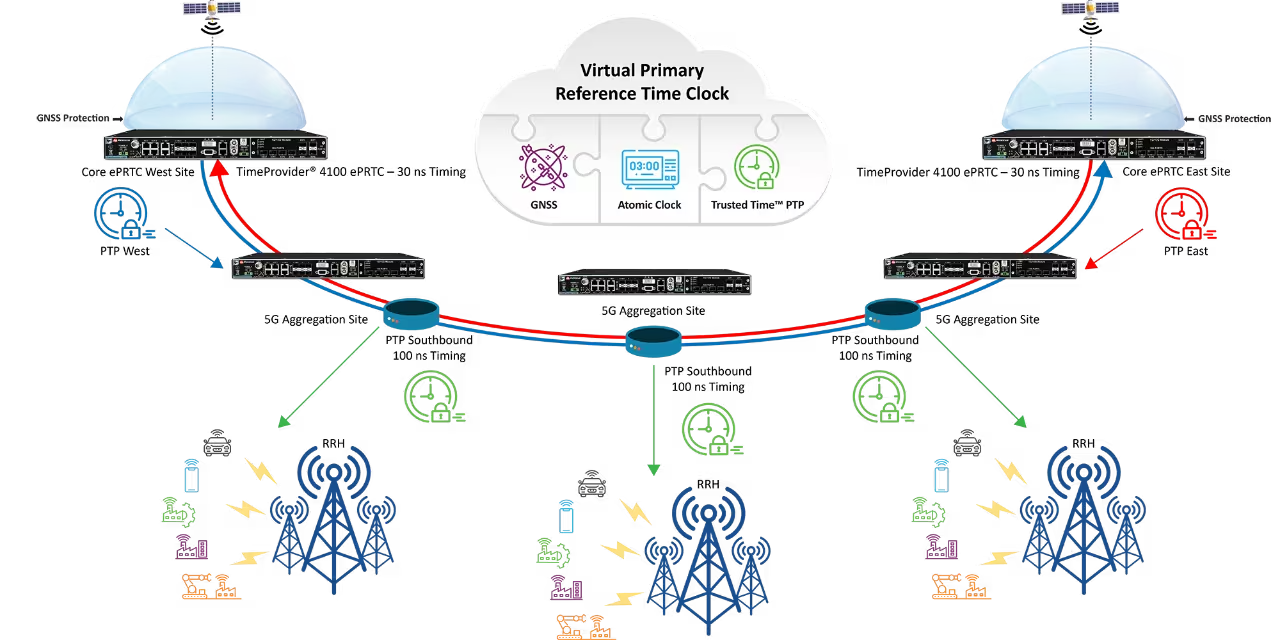
\includegraphics[width=0.8\textwidth]{img/5G.png}
    \end{figure}

\end{frame}



\begin{frame}{Space experiments}

    Space versions of CSACs are being developed for scientific missions and data collection.

    SPATIUM (Space Precision Atomic-clock Timing Utility Mission) is a mission with the objective to model the ionosphere TEC (Total Electron Content) based on multipoint measurements formed by a constellation of small satellites.

    \begin{figure}
        \centering
        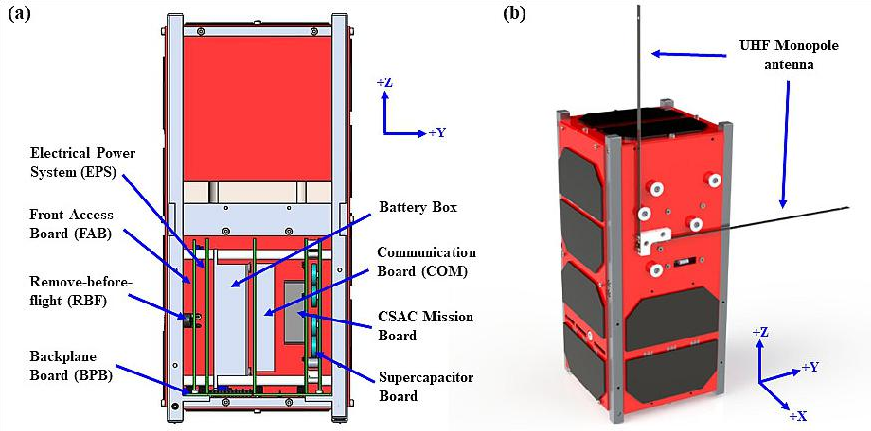
\includegraphics[width=0.8\textwidth]{img/SPATIUM.png}
    \end{figure}

\end{frame}